%==============================================================================
%== Poster: Hoạch định chuyển động cho Rô-bốt sử dụng Tối ưu Lồi
%== Portrait A0 – 2 cột – phong cách tối giản
%== HK252 – Khoa KHKT Máy tính, ĐHQG TP.HCM
%==============================================================================

\documentclass[final]{beamer}
\usepackage[orientation=portrait,size=a0,scale=1.20]{beamerposter}
\geometry{hmargin=2.5cm,vmargin=1.5cm}

\usepackage[utf8]{inputenc}
\usepackage[vietnamese]{babel}
\usepackage[T5]{fontenc}
\usepackage{amsmath,amssymb,mathtools}
\usepackage{booktabs,array}
\usepackage{graphicx}
\usepackage{float}
\usepackage{tikz}
\usetikzlibrary{arrows.meta,shapes.geometric,positioning,fit,calc}
\usepackage{tcolorbox}
\tcbuselibrary{most}
\usepackage{ragged2e}
\usepackage{enumitem}

\linespread{1.08}

% ── Bảng màu tùy chỉnh ───────────────────────────────────────
\definecolor{softmint}{HTML}{A8D5BA}
\definecolor{aquamarine}{HTML}{7FFFD4}   % xanh lá mint chủ đạo
\definecolor{softcoral}{HTML}{FFB3A7}    % san hô nhạt
\definecolor{softlavender}{HTML}{C8B4E8} % tím lavender nhạt
\definecolor{softyellow}{HTML}{FFF176}   % vàng chanh nhạt
\definecolor{softpeach}{HTML}{FFCC99}    % đào nhạt
\definecolor{softsky}{HTML}{90CAF9}      % xanh trời nhạt

\graphicspath{
  {../Report Source/experiments/image/}
  {../Report Source/experiments/image/dms/}
  {figures/}
}

\usetheme{sharelatex}
\setlength{\columnsep}{45pt}

% Hộp công thức – nền softmint nhạt, viền softmint đậm
\newtcolorbox{mathbox}{
  enhanced,
  colback=softmint!28, colframe=softmint!85,
  boxrule=1.6pt, arc=5pt,
  left=5pt, right=5pt, top=3pt, bottom=3pt
}

% Hộp thông điệp – nền vàng chanh, viền san hô
\newtcolorbox{keybox}{
  enhanced,
  colback=softyellow!55, colframe=softcoral!90,
  boxrule=2pt, arc=5pt,
  left=7pt, right=7pt, top=4pt, bottom=4pt
}

% Hộp placeholder – đào nhạt trung tính
\newtcolorbox{placeholderbox}{
  enhanced,
  colback=softpeach!25, colframe=softpeach!65,
  boxrule=1pt, arc=4pt,
  left=6pt, right=6pt, top=4pt, bottom=4pt
}

% Hộp kết luận – tím lavender nhạt, thanh bên aquamarine
\newtcolorbox{conclusionbox}{
  enhanced,
  colback=softlavender!32, colframe=softlavender!80,
  borderline west={3.5pt}{0pt}{aquamarine!90},
  boxrule=0.8pt, arc=4pt,
  left=10pt, right=7pt, top=5pt, bottom=5pt
}

% Hộp tài liệu tham khảo – xanh trời, nhãn tiêu đề nổi
\newtcolorbox{refbox}{
  enhanced,
  colback=softsky!30, colframe=softsky!80,
  boxrule=1.3pt, arc=5pt,
  left=7pt, right=7pt, top=8pt, bottom=5pt,
  title={\small\bfseries\color{black} Tài liệu tham khảo},
  fonttitle=\small\bfseries,
  attach boxed title to top left={yshift=-2.5mm, xshift=6mm},
  boxed title style={
    colback=softsky!80, colframe=softsky!80,
    arc=3pt, boxrule=0pt,
    left=4pt, right=4pt, top=1.5pt, bottom=1.5pt
  }
}

%==============================================================================
\title[Ngày hội kỹ thuật HK252 --- Khoa KHKT Máy tính, ĐHQG TP.HCM]{%
  Hoạch định chuyển động cho Rô-bốt\\[0.3ex]sử dụng Tối ưu Lồi%
}
\author{%
\textbf{Mã đề tài:} HK252-DATN-028 \quad | \quad \textbf{GVHD:} PGS.TS.\ Lê Hồng Trang \& ThS.\ Trương Quỳnh Chi%
\\ % \qquad% 
\textbf{SVTH:} Nguyễn Trần Đăng Khoa (2211635) \& Hồ Đăng Khoa (2211588)%
}
\institute[VNU-HCM]{%
  Khoa Khoa học và Kỹ thuật Máy tính --- Trường Đại học Bách khoa --- ĐHQG TP.HCM%
  \qquad HK252%
}
\date{\today}

%==============================================================================
\begin{document}
\begin{frame}[t]
  \begin{columns}[t,totalwidth=\textwidth]
    \begin{column}{0.48\textwidth}
      \justifying

      %======================================================================
      \section{Bài toán Hoạch định Chuyển động}

      % ---- FIX 1: Hàm mục tiêu rõ ràng + tính phi lồi (thesis eq. 4.1–4.2) ----

      \textbf{Bài toán:} Sinh quỹ đạo cho rô-bốt trong môi trường có vật cản, đảm bảo (i) tránh va chạm, (ii) trơn (liên tục bậc cao), (iii) khả thi về mặt động lực học.

      \textbf{Hàm mục tiêu:}
      \begin{mathbox}
        \[
          \min_{x(\cdot),\,T}\;
          \ell\bigl(x(\cdot),T\bigr)
          \;:=\;
          \underbrace{a\,\Phi(T)}_{\text{chi phí thời gian}}
          +\;\sum_{m=1}^{M} b_m
          \underbrace{\int_0^T\!\left\|\frac{d^m x}{dt^m}\right\|^2\!dt}_{%
          m{=}1:\,\text{quãng đường};\;
          m{=}2:\,\text{năng lượng}\,(a)}
        \]
      \end{mathbox}

      \textbf{Ràng buộc:}
      \[
        \begin{alignedat}{3}
           & x(0)=x_{\mathrm{start}},\quad                                                                     &  & x(T)=x_{\mathrm{goal}} \\
           & x(t)\in\mathcal{C}_{\mathrm{free}},\quad                                                          &  & \forall t\in[0,T]
          \quad\longleftarrow\;\textbf{phi lồi}\;\Rightarrow\;\text{NP-hard}                                                               \\
           & \tfrac{d^k x}{dt^k}(t)\in \underbrace{\mathcal{D}_k}_{\footnotesize\text{RB vật lý bậc } k},\quad &  & k=1,\ldots,K
          \quad(\text{giới hạn }v,\,a,\,\ldots)                                                                                            \\
           & T_{\min}\leq T \leq T_{\max}
        \end{alignedat}
      \]

      % {\small $a,b_m>0$: hệ số trọng số;\quad
      % $\Phi(T)$: chi phí liên quan thời gian;\quad
      % $\mathcal{D}_k$: tập ràng buộc vật lý bậc~$k$.}

      \begin{keybox}
        \centering
        % \textbf{Tính phi lồi:}\;
        $\mathcal{C}_{\mathrm{free}}=\mathcal{C}\setminus\mathcal{O}$,\;
        $\mathcal{O}$ hợp các vật cản
        $\;\Rightarrow\;$
        ràng buộc $x(t)\in\mathcal{C}_{\mathrm{free}}$ \textbf{phi lồi}\\[0.25em]
        $\mathcal{C}_{\mathrm{free}} \approx \displaystyle\bigcup_{i=1}^{N} Q_i,\quad Q_i \text{ lồi}$
        \qquad
        {\small\textbf{Biến bài toán phi lồi thành đồ thị GCS giải được}}
      \end{keybox}

      %======================================================================
      % ---- FIX 2: Bảng so sánh 3 phương pháp phân hoạch (thesis Bảng 4.1) ----
      \section{Phân hoạch Không gian Tự do}

       {\small
        \renewcommand{\arraystretch}{1.15}
        \begin{tabular}{@{}p{9cm}p{13.5cm}p{14cm}@{}}
          \toprule
          \textbf{Phương pháp} & \textbf{Ưu điểm}                                                               & \textbf{Nhược điểm} \\
          \midrule
          \textbf{ACD}\newline
          {\footnotesize Approx.\ Convex Decomp.}
                               & Không cần vật cản lồi; bao phủ $\mathcal{C}_\mathrm{free}$; phù hợp polygon 2D
                               & Xấp xỉ (dung sai $\tau$); heuristic; số vùng khó kiểm soát                                           \\[4pt]
          \textbf{IRIS}\newline
          {\footnotesize Iter.\ Inflation by SDP}
                               & Vùng lồi chính xác trong $\mathbb{R}^n$; mở rộng tốt (QP+SDP)
                               & Điểm mầm thủ công; cần vật cản lồi; không tự bao phủ                                                 \\[4pt]
          \textbf{VCC}\newline
          {\footnotesize Visibility Clique Cover}
                               & Tự động đặt điểm mầm; ít vùng hơn IRIS; bao phủ tự động
                               & Lấy mẫu dày không gian hẹp; MAXCLIQUE giải gần đúng (ILP)                                            \\
          \bottomrule
        \end{tabular}
       }

      %======================================================================
      \vspace{0.4em}
      % ---- FIX 3: Bézier — thêm hàm mục tiêu, kỹ thuật phối cảnh, bao lồi ----
      \section{Hướng 1: GCS-Bézier}
      \begin{mathbox}
        \[
          \min_{\{y_e,\,r_{v,k},\,h_{v,k}\}}
          \sum_{e\in E}
          \underbrace{\tilde{\ell}_e\!\bigl(z_{e,u},z_{e,v},y_e\bigr)}_{\text{perspective của }\ell_e},
          \qquad
          z_{e,\cdot}=y_e\,x_{\cdot}
        \]
        \[
          \ell_e = \underbrace{w_t T_v}_{\text{thời gian}}
          + \underbrace{\textstyle\int_0^{T_v}\!\|\dot{r}\|^2 dt}_{\text{năng lượng}}
          + \underbrace{\textstyle\sum_k\|\ddot{r}_{v,k}\|^2}_{\text{độ giật (jerk)}}
        \]
      \end{mathbox}

      \textbf{Kỹ thuật phối cảnh} chuyển MICP sang MI-SOCP giải hiệu quả:
      \[
        \underbrace{\dot{r}_{v,k}\in\dot{h}_{v,k}\mathcal{D}}_{\substack{\text{vận tốc dạng phối cảnh}\\\text{lồi theo }(\dot{r}_{v,k},\dot{h}_{v,k})}}
        \xrightarrow{\;z_{e,\cdot}=y_e x_\cdot\;}
        \text{MICP}
        \xrightarrow{\;\text{relaxation}\;}
        \text{MI-SOCP}
      \]

      \begin{center}
        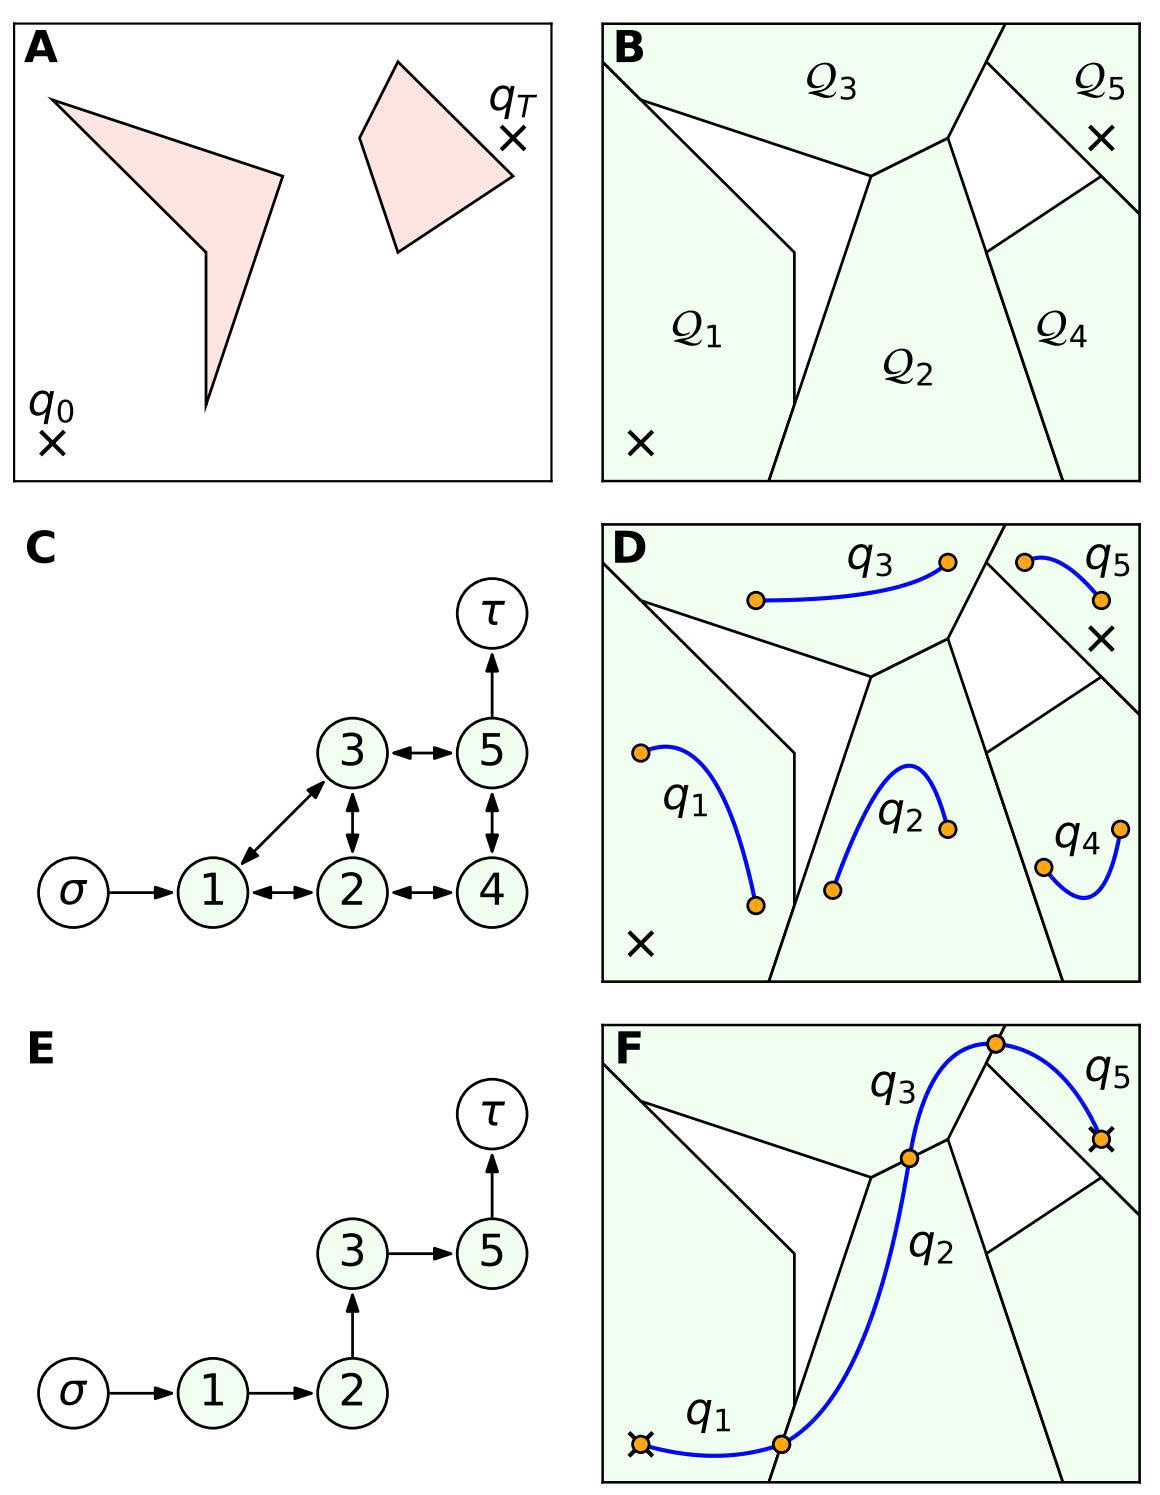
\includegraphics[width=0.82\linewidth]{beziergcs_pipeline.jpg}\\[-2pt]
        {\footnotesize GCS-Bézier: đồ thị lồi $\to$ relaxation $\to$ quỹ đạo mượt
        \textup{(Marcucci et al., 2023)}}
      \end{center}

      %======================================================================
      \vspace{0.4em}
      % ---- FIX 4: DMS — OCP rõ ràng + hàm mục tiêu tổng quát
      \section{Hướng 2: GCS-DMS}

      \begin{mathbox}
        \[
          \min\sum_{v\in V_r} p_v\!\left[
          \underbrace{J_v(s_v^-,w_v,\Delta_v)}_{\text{chi phí cục bộ vùng }v}
          +\int_0^1\!\Delta_v\,\mu_v\,
          \underbrace{\phi_v\!\bigl(x_v(\tau)\bigr)}_{\text{log-barrier an toàn}}
          d\tau
          \right]
        \]
        \[
          J_v:=a\Delta_v
          +\int_0^1\!\!\Delta_v\!\left(
          w_L\!\left\|\tfrac{1}{\Delta_v}\tfrac{dq_v}{d\tau}\right\|^2
          +w_E\|u_v\|^2\right)d\tau
        \]
      \end{mathbox}
      {\small
      $p_v\!\in\!\{0,1\}$: kích hoạt vùng;\;\;
      $\Delta_v$: thời lượng đoạn;\;\;
      $\phi_v(x)\!=\!-\!\sum_j\!\log\bigl((b_v)_j\!-\!(A_vx)_j\bigr)$;\;\;
      $\mu_v$: trọng số barrier.
      }

      \textbf{Ràng buộc defect} (liên tục động lực học):
      \[
        s_v^+ - F_v(s_v^-,w_v,\Delta_v)=0,\quad\forall v\in V_r
        \quad\bigl(F_v=x_v(1):\;\text{tích phân IVP}\bigr)
      \]

      \begin{center}
        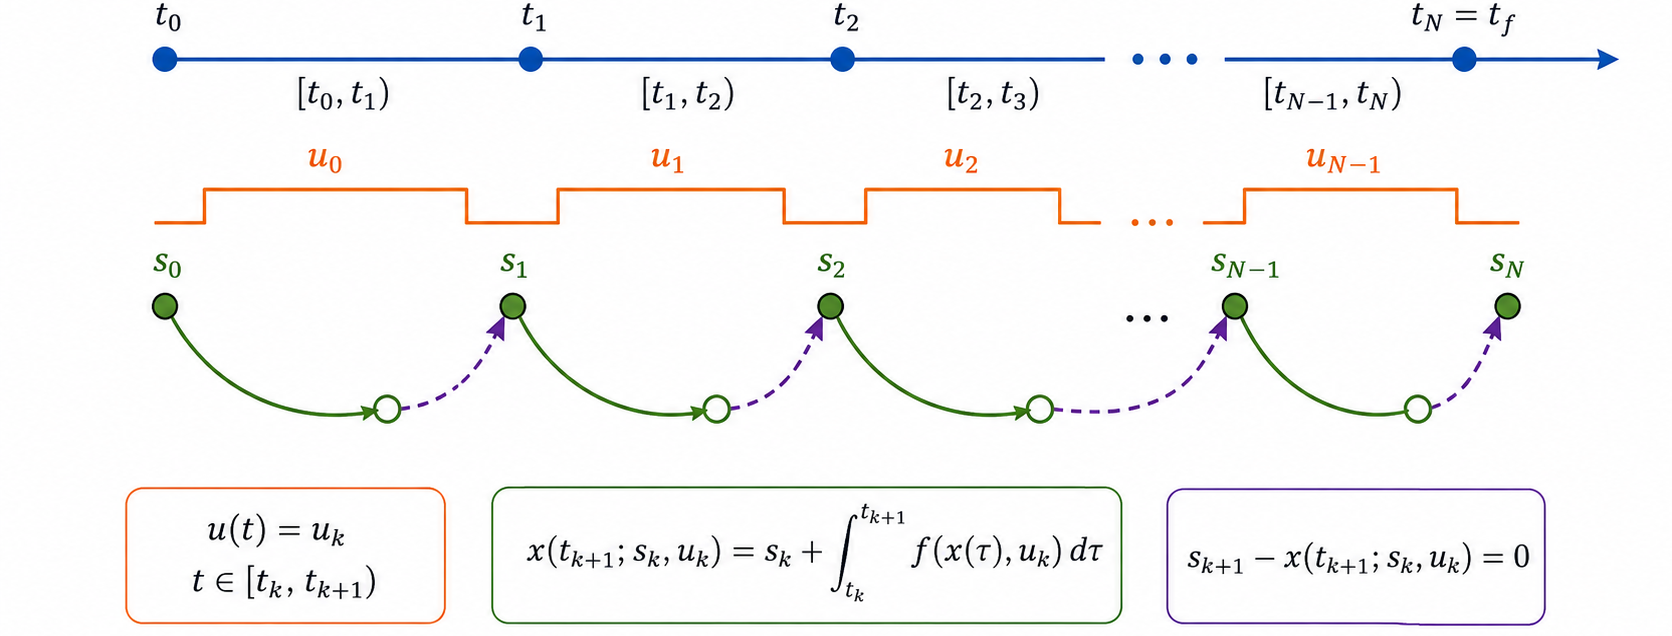
\includegraphics[width=0.82\linewidth]{dms_v2.png}\\[-2pt]
        % {\footnotesize GCS-DMS: OCP $\to$ MINLP giải bằng NLP (IPOPT)}
      \end{center}
    \end{column}

    %======================================================================%
    % ---- Cột 2: Kết quả, so sánh, kết luận ----%

    \begin{column}{0.48\textwidth}
      \justifying

      %======================================================================
      \section{Kết quả: GCS-DMS --- Unicycle Dynamics}
      \begin{center}
        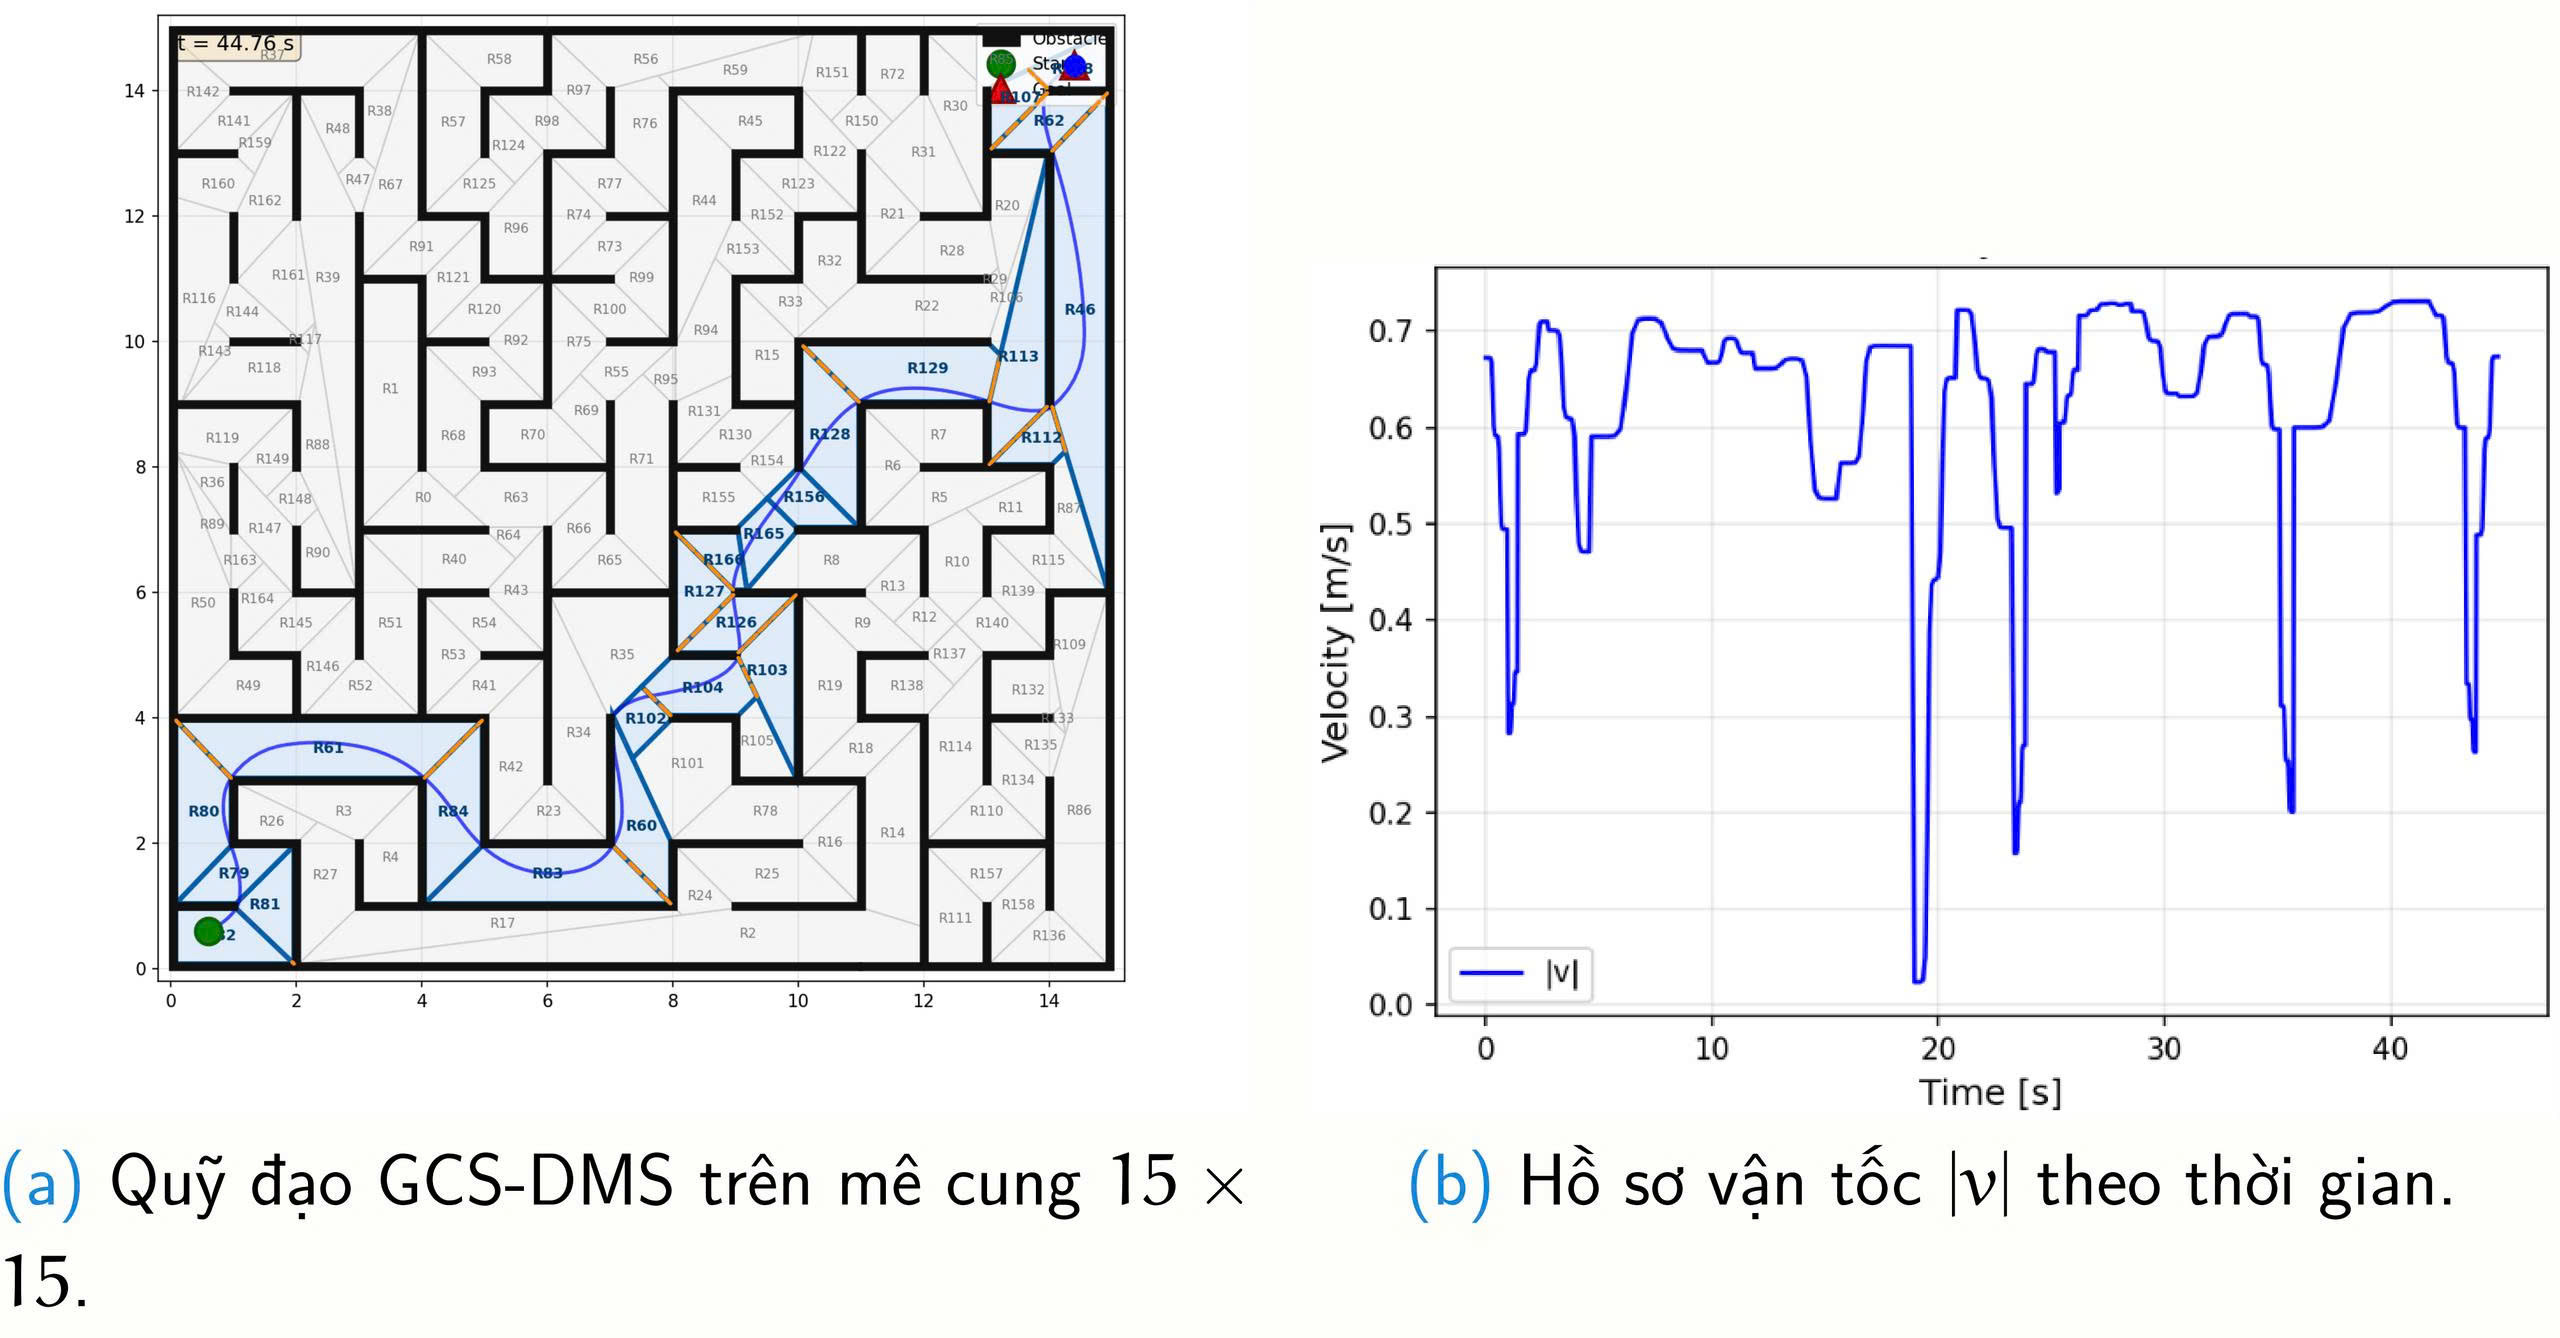
\includegraphics[width=0.82\linewidth]{maze-dms.jpg}\\[-2pt]
        {GCS-DMS: OCP $\to$ MINLP giải bằng NLP (IPOPT) - khả thi động lực học}
      \end{center}

      \begin{minipage}[t]{0.47\linewidth}
        \vspace{0pt}
        \subsection{Môi trường 2D đơn giản}

        \begin{center}
          \small\renewcommand{\arraystretch}{1.2}
          \begin{tabular}{lr}
            \toprule
            \textbf{Chỉ số} & \textbf{Giá trị}        \\
            \midrule
            Vùng kích hoạt  & 9                       \\
            Duration        & 25.47 s                 \\
            Thời gian giải  & 17.94 s                 \\
            Defect dynamics & $2.5\!\times\!10^{-11}$ \\
            Connection gap  & $1.1\!\times\!10^{-10}$ \\
            Violation       & $7.1\!\times\!10^{-8}$  \\
            \bottomrule
          \end{tabular}
        \end{center}
      \end{minipage}
      \hfill
      \begin{minipage}[t]{0.50\linewidth}
        \vspace{0pt}
        \subsection{Mê cung $15\!\times\!15$ --- 4 seeds}

        \begin{center}
          \small\renewcommand{\arraystretch}{1.15}
          \begin{tabular}{@{}clcrr@{}}
            \toprule
            \textbf{Seed} & \textbf{An toàn} & \textbf{Vùng}
                          & \textbf{Cost}    & \textbf{Defect/Gap}                            \\
            \midrule
            4             & Log-barrier      & 24                  & 92.6  & ${\sim}10^{-9}$  \\
            17            & Lưới h.f.        & 27                  & 113.5 & ${\sim}10^{-9}$  \\
            18            & Lưới h.f.        & 33                  & 95.8  & ${\sim}10^{-9}$  \\
            20            & Log-barrier      & 44                  & 150.6 & ${\sim}10^{-10}$ \\
            \bottomrule
          \end{tabular}
        \end{center}
      \end{minipage}

      \vspace{0.6em}
      %======================================================================
      \section{Kết quả: GCS-Bézier --- Mê cung $25\!\times\!25$}
      \begin{center}
        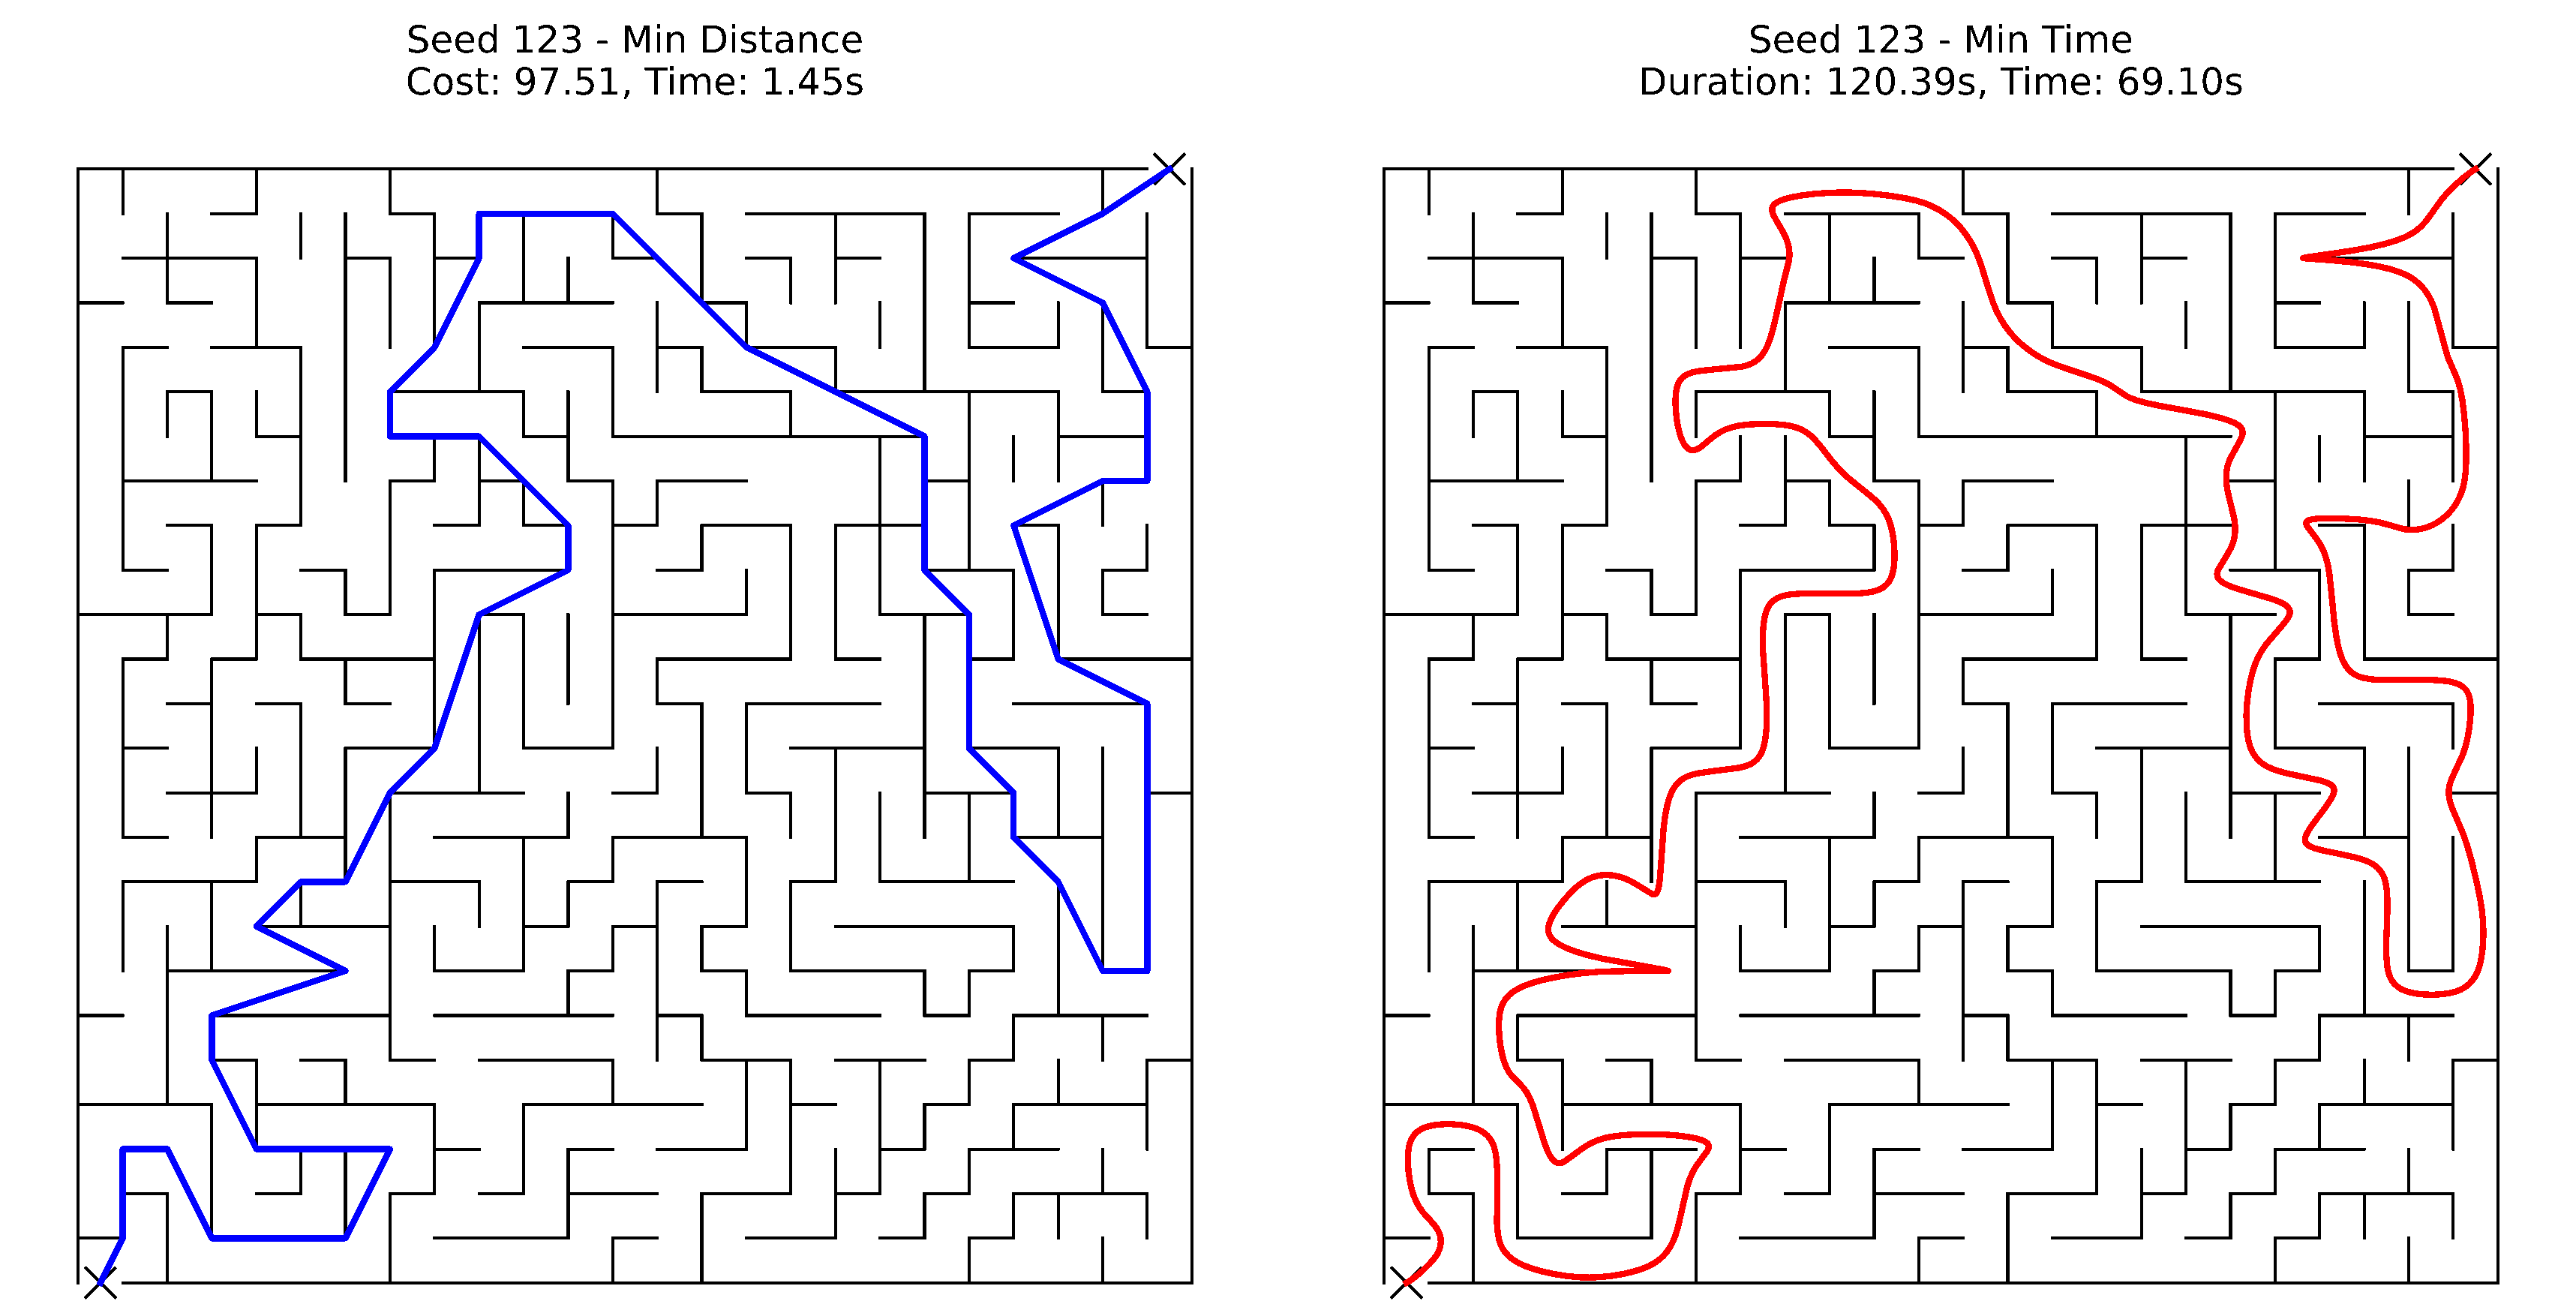
\includegraphics[width=0.82\linewidth]{maze-gcsbezier.png}\\[-2pt]
        {Bézier bậc $d=6$, liên tục $C^2$ tại các điểm nối giữa vùng lồi. Relaxation SOCP luôn cho nghiệm binary xấp xỉ tốt - không cần rounding heuristic}
      \subsection{Kết quả chi tiết}
      \end{center}
      \begin{center}
        \small\renewcommand{\arraystretch}{1.2}
        \begin{tabular}{lrr}
          \toprule
          \textbf{Chỉ số} & \textbf{Linear GCS} & \textbf{Bézier GCS} \\
          \midrule
          Solve time (TB) & 1.28 s              & 85.22 s             \\
          Cost (TB)       & 71.88               & 88.03               \\
          Cost ratio      & 0.82$\times$        & 1.00$\times$        \\
          \bottomrule
        \end{tabular}
      \end{center}
      
      \vspace{0.6em}
      %======================================================================
      \section{So sánh \& Kết luận}

      \begin{center}
        \small\renewcommand{\arraystretch}{1.25}
        \begin{tabular}{@{}p{5cm}p{10cm}p{10cm}@{}}
          \toprule
          \textbf{Tiêu chí} & \textbf{GCS-Bézier}                     & \textbf{GCS-DMS}             \\
          \midrule
          Mô hình
                            & Bézier trên vùng lồi
                            & Direct Multiple Shooting                                               \\[2pt]

          Bài toán          & MISOCP $\rightarrow$ SOCP               & MIOCP $\rightarrow$ MINLP    \\[2pt]

          Điểm mạnh
                            & Nhanh, lồi, quỹ đạo mượt $C^2$
                            & Khả thi động lực học, có điều khiển $u$                                \\[2pt]

          Hạn chế           & Chưa ràng buộc dynamics đầy đủ          & Chậm, phi lồi, nhạy khởi tạo \\[2pt]

          Phù hợp           & Planning hình học nhanh                 & Planning có dynamics thực    \\

          \bottomrule
        \end{tabular}
      \end{center}

      \vspace{0.5em}
      \begin{conclusionbox}
        \textbf{Kết luận:} GCS-Bézier là convex relaxation của MICP — tight khi các vùng lồi đủ lớn và ít overlap.
        GCS-DMS bổ sung khả năng mô hình hoá nonlinear dynamics nhưng là NLP non-convex với nguy cơ local minima
        — phù hợp nhất khi warm-start từ GCS-Bézier.
      \end{conclusionbox}

      \vspace{0.8em}
      %======================================================================
      \begin{refbox}
        \begin{enumerate}[label={[\arabic*]}, leftmargin=*, itemsep=2pt, topsep=3pt,
            labelsep=4pt]
          \small
          \item T.~Marcucci et al., ``Motion Planning around Obstacles with Convex
                Optimization,'' \textit{Science Robotics}, 2023.
          \item J.~M.~Lien \& N.~M.~Amato, ``Approximate Convex Decomposition of Polygons,''
                \textit{CGTA}, 2006.
          \item M.~Diehl et al., ``Fast Direct Multiple Shooting Algorithms for Optimal Robot
                Control,'' \textit{Springer}, 2006.
        \end{enumerate}
      \end{refbox}

      %======================================================================
    \end{column}
  \end{columns}
\end{frame}
\end{document}
